\begin{frame}
\frametitle{Fast File System}
\begin{itemize}
  \item Fast File System - ФС разработанная для замены ФС созданной Кеном Томпсоном:
    \begin{itemize}
      \item ФС от Томпсона даже не пыталась поддерживать локальность и бороться с фрагментацией;
      \item ее производительность была ужасна и со временем становилась хуже;
      \item группа исследователей в Berkely разработала ФС решающую эти проблемы в 1984;
    \end{itemize}
  \item Основная идея Fast File System учитывать специфику дискового доступа:
    \begin{itemize}
      \item располагать файлы последовательно;
      \item избегать позиционирований головки диска;
      \item Marshall Kirk McKusick, William N. Joy, Samuel J. Leffler, Robert S. Fabry "A Fast File System for UNIX"
    \end{itemize}
\end{itemize}
\end{frame}

\begin{frame}
\frametitle{Разметка диска в FFS}
\begin{figure}
  \centering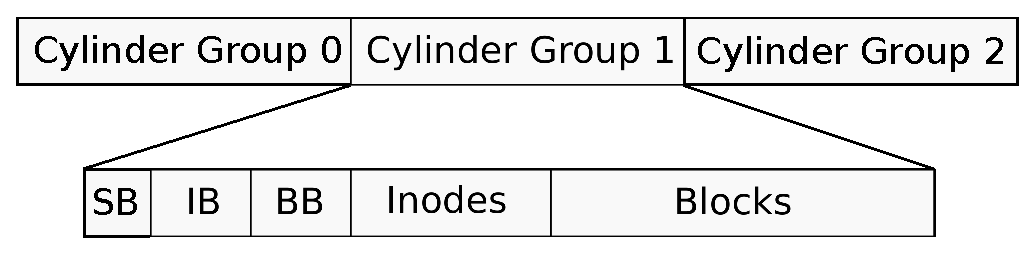
\includegraphics[width=.6\linewidth]{ffs-layout}
  \caption{FFS Layout}
\end{figure}
\begin{itemize}
  \item Все пространство разбито на цилиндровые группы для поддержки локальности;
  \item каждая группа содержит копию суперблока (SB) с параметрами ФС;
  \item IB и BB - битовая карта свободных/занятых inode и блоков внутри группы;
  \item inodes - таблица индексных узлов (Index Nodes);
\end{itemize}
\end{frame}

\begin{frame}
\frametitle{Индексный узел}
\begin{itemize}
  \item Inode представляет сущности ФС (файлы/каталоги/специальные файлы):
    \begin{itemize}
      \item inode хранит информацию о блоках файла;
      \item inode хранит атрибуты файла;
      \item inode не хранит имя файла - один и тот же inode может соответствовать нескольким именам;
    \end{itemize}
  \item Количество индексных узлов определяется в момент форматирования;
\end{itemize}
\end{frame}

\begin{frame}
\frametitle{Политика выделения ресурсов}
\begin{itemize}
  \item В FFS есть два ресурса, которые нужно выделять: Inode и блоки диска;
  \item ФС старается выделять inode-ы файлов одного каталога в одной группе цилиндров
    \begin{itemize}
      \item команда ls требует обращения к inode, таким образом ускоряем ls;
    \end{itemize}
  \item ФС распределяет inode-ы каталогов равномерно по группам;
  \item ФС старается выделять блоки одного файла в одной группе
    \begin{itemize}
      \item для больших файлов стараемся выделять большие порции файла в одной группе;
      \item порции файлов распределяются по разным группам;
    \end{itemize}
\end{itemize}
\end{frame}

\begin{frame}
\frametitle{Блоки файла}
\begin{figure}
  \centering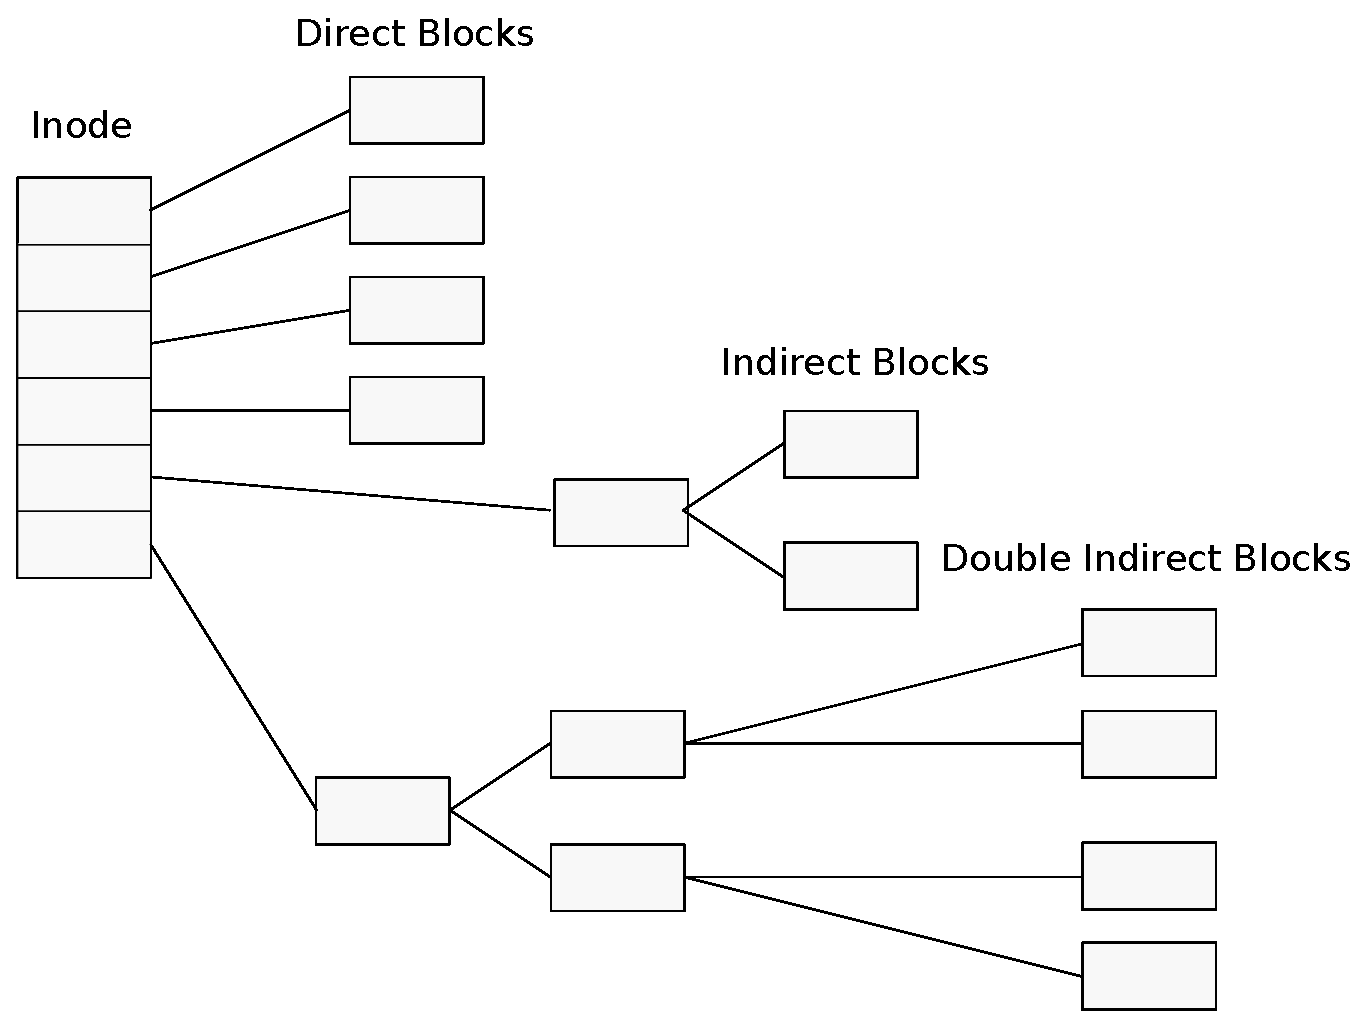
\includegraphics[width=.6\linewidth]{ffs-inode}
  \caption{FFS Inode Blocks}
\end{figure}
\end{frame}
